%% ============================================================
%%  Chapter 3 — Compositional and Chemical Control of Volatile
%%              Polymer-Electrolyte Memristive Dynamics
%%
%%  Author : Carlos David Prado-Socorro
%%  Date   : June 2026
%%  Institution : ICMol, Universitat de València
%%
%%  Compile with: latexmk -pdf  (standalone) or via thesis.tex
%%  Plan + evidence: handouts/10_chapter3_comparative_plan.md,
%%                   handouts/08_chapter3_4_claims_audit.md
%% ============================================================

%% ---- Standalone preamble (skipped when \include'd from thesis.tex) ----
\ifdefined\thesismode\else
  \documentclass[12pt, twoside]{report}
  \usepackage{thesis-format}
  \addbibresource{../bibliography/references.bib}
  \begin{document}
  \setcounter{chapter}{2}     % This is Chapter 3 when built standalone
\fi

%% --- Shared macros (\providecommand: harmless if ch.2 already declared them) ---
\providecommand{\SY}{\textit{Super Yellow}}
\providecommand{\Hybrane}{\textit{Hybrane}}
\providecommand{\PEO}{PEO}
\providecommand{\TMPE}{TMPE}
\providecommand{\LiTf}{LiOTf}
\providecommand{\NaTf}{NaOTf}
\providecommand{\KTf}{KOTf}
\providecommand{\TFSI}{TFSI}
\providecommand{\ITO}{ITO}
\providecommand{\twoterminal}{two-terminal}
\providecommand{\figplaceholder}[2]{%
  \setlength{\fboxsep}{0pt}%
  \fbox{\parbox[c][#1][c]{0.85\linewidth}{%
    \centering\itshape [Figure placeholder]\\[2pt]
    #2\\[2pt]
    \footnotesize\upshape to be generated from data --- see
    \texttt{handouts/10\_chapter3\_comparative\_plan.md}%
  }}%
}

%% ============================================================
\chapter{Compositional and Chemical Control of Volatile Polymer-Electrolyte Memristive Dynamics}\label{ch:comparative}
%% ============================================================

%% ------------------------------------------------------------
\section{Introduction and Scope}\label{sec:ch3_intro}
%% ------------------------------------------------------------

\Cref{ch:poc} established, on a single fully characterised \SY{}/\Hybrane{}/\LiTf{} device, that a three-component polymer-electrolyte composite supports the full set of memristive functions in one \twoterminal{} platform. The natural next question --- and the subject of this chapter --- is how the \emph{dynamics} of these devices respond to deliberate changes in the composite, so that the volatile, fading-memory behaviour can be treated as something to be engineered rather than merely observed.

Three families of measurement recur on the same 2-T geometry throughout this chapter and the next, and are introduced here as a named set. They are (i) current--voltage hysteresis, which reports the steady-state switching window; (ii) potentiation as a function of the number of applied write pulses, which reports how the conductance is built up; and (iii) depotentiation as a function of the delay before read-out, which reports how a written state fades. These three measurements are the shared, abundant basis of the comparative work. The richer single-device synaptic protocols of \cref{ch:poc} --- excitatory post-synaptic current, separated short- and long-term memory, and spike-timing dependent plasticity --- are \emph{not} repeated across the families studied here; where they are invoked, they are used only as prior evidence from the Chapter~\ref{ch:poc} device and are labelled as such.

\paragraph{Claim discipline.} A central feature of this chapter, stated here so that the reader can hold it throughout, is that its results fall into two evidential tiers. The \textbf{composition} axis --- variation of the ion-transport polymer and salt mass fractions in the \SY{}/\PEO{}/\LiTf{} system --- is supported by a replicated design (typically two to four nominally identical devices per composition cell) and is presented as a \emph{quantitative} result. The \textbf{chemistry} axis --- variation of the ion-transport host, the salt anion, and the alkali cation --- is supported, after data-quality screening, by at most one or two devices per matched cell; it is therefore presented as an \emph{illustrative} landscape, with sample sizes stated explicitly and no claim of statistical power. A third, methodological result establishes that the \emph{drive protocol} itself sets the apparent fading-memory timescale, which both explains why the chemistry comparisons must be read cautiously and provides a design rule for any future comparative study.

%% ------------------------------------------------------------
\section{Materials, Devices, and Measurement Protocol}\label{sec:ch3_materials}
%% ------------------------------------------------------------

The devices retain the architecture of \cref{ch:poc}: a vertical \twoterminal{} sandwich of \ITO{} (bottom, transparent), a solution-processed composite active layer, and a thermally evaporated silver top electrode, with a junction area of \SI{8.25e-2}{\centi\meter\squared}. \SY{} is retained as the semiconducting component in every device of this chapter, so that the electronic-transport role is held fixed and the variation is confined to the ion-transport phase.

Two design axes are varied. The \emph{composition} axis varies the mass fraction of the ion-transport polymer poly(ethylene oxide) (\PEO{}) and of the lithium triflate salt (\LiTf{}) relative to the semiconductor. The \emph{chemistry} axis substitutes the ion-transport host (\PEO{} or the hyperbranched polyether \TMPE{}), the salt anion (triflate or bis(trifluoromethanesulfonyl)imide, \TFSI{}), and the alkali cation (\ce{Li+}, \ce{Na+}, \ce{K+}, as the triflate or \TFSI{} salt). All devices reported quantitatively use the silver electrode; the small number of gold-electrode devices in the archive are held separate, because the electrode is a confounding variable (\cref{sec:ch3_protocol}).

\paragraph{Drive and read protocol.} Because the comparisons below turn on it, the electrical protocol is stated explicitly. Potentiation and delay-time measurements use a fixed train of \num{30} write pulses with a fixed inter-pulse interval of \SI{0.103}{\second}; the standard amplitude across the modern corpus is a \SI{4}{\volt} write pulse with a \SI{2}{\volt} read. An older device generation used a \SI{6}{\volt} write with a \SI{3}{\volt} read; the two protocols are never pooled (\cref{sec:ch3_protocol}). The read voltage is above the ionic activation threshold of the system established in \cref{ch:poc}, a point returned to in \cref{sec:ch3_protocol}.

%% ------------------------------------------------------------
\section{Methods of Analysis}\label{sec:ch3_methods}
%% ------------------------------------------------------------

Hysteresis curves are summarised by the on--off conductance ratio and by a normalised loop area; potentiation curves by the per-decade growth of the conductance ratio with pulse number, by the peak ratio, and by whether the response turns over (decreases) at the highest pulse counts; and depotentiation curves by a fading-memory time constant.

For the depotentiation (fading-memory) decay, the conductance relaxation is described, as in \cref{ch:poc}, by a Kohlrausch (stretched-exponential) function
\begin{equation}
  \label{eq:ch3_kohlrausch}
  \Delta G(t_{\mathrm{wait}}) = \Delta G_0\,\exp\!\left[-\left(\frac{t_{\mathrm{wait}}}{\tau}\right)^{\beta}\right] + \Delta G_\infty,
\end{equation}
with characteristic relaxation time \(\tau\), stretch exponent \(0 < \beta \le 1\), initial change \(\Delta G_0\), and residual \(\Delta G_\infty\)~\cite{Sturman2003}. Two practical points follow from the data. First, the eight-to-thirteen-point decay curves often under-constrain \(\beta\) and \(\tau\) jointly; the fitted \(\tau\) is therefore reported only where the fit is well identified, and a robust, model-free half-enhancement time \(t_{1/2}\) (the delay at which the conductance enhancement has fallen to half its initial value) is used as the primary timescale. Where both are available they agree. Second, fitted \(\beta\) values lie predominantly in the range \numrange{0.6}{0.9}, i.e. genuinely stretched relaxation, consistent with the heterogeneous distribution of activation barriers invoked in \cref{ch:poc}.

\paragraph{Data-quality control.} Two screening layers are applied before any number is reported, both recorded so that the analysis is reproducible. Individual measurements that are erratic or non-physical are flagged and excluded. In addition, a per-device visual review of the recorded curves was carried out; the resulting verdicts --- whether a curve is used as measured, cleaned by removing identified anomalous points, or discarded --- together with the exact points retained, are stored in a curation registry and applied automatically by the analysis scripts, rather than being made ad hoc. The fitted timescale obtained directly from the instrument-side pipeline was found not to be robust to such anomalous points, so all timescales reported here are recomputed after this screening.

%% ------------------------------------------------------------
\section{Composition Control of the Dynamics}\label{sec:ch3_composition}
%% ------------------------------------------------------------

The quantitative core of this chapter is the \SY{}/\PEO{}/\LiTf{} composition grid, in which the \PEO{} mass fraction is varied over \numlist{0.3;0.6;1.2} and the salt mass fraction over \numlist{0.045;0.09;0.18}, with two to four nominally identical silver-electrode devices per cell under the common \SI{4}{\volt}/\SI{2}{\volt} protocol. Three trends, mutually consistent and each visible across the grid, define the result.

\begin{figure}[t]
  \centering
  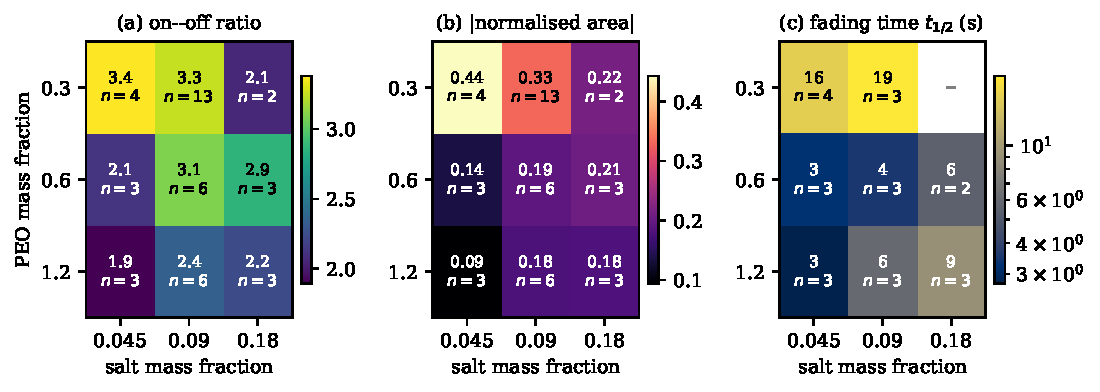
\includegraphics[width=\linewidth]{../figures/chapter3/composition_heatmaps.pdf}
  \caption[Composition control of the memristive dynamics]{Composition control of the steady-state and dynamical response of \SY{}/\PEO{}/\LiTf{} devices. The switching window (a, b) and the fading-memory time (c) both decrease as the \PEO{} mass fraction increases at fixed salt content.}
  \label{fig:ch3_composition_heatmaps}
\end{figure}

First, the steady-state switching window contracts as the \PEO{} fraction rises. At fixed salt mass fraction \num{0.09}, the median on--off ratio falls from \(\approx 3.3\) at \PEO{}~\num{0.3} to \(\approx 2.4\) at \PEO{}~\num{1.2}, and the normalised loop area falls correspondingly from \(\approx 0.33\) to \(\approx 0.18\); the activation voltage is, by contrast, essentially flat across the whole grid (\SIrange{2.2}{2.4}{\volt}), indicating that composition tunes how \emph{much} the conductance moves rather than the voltage at which it begins to move. The widest window in the grid sits in the low-\PEO{} row, with the largest loop area at the low-salt corner (\PEO{}~\num{0.3}, salt~\num{0.045}: area \(\approx 0.44\)); the per-sweep on--off ratio is strongly right-skewed there (cell median \(\approx 3.4\) but individual sweeps reaching \(\sim 40\)), so robust cell medians rather than means are reported throughout to avoid letting a few outlying sweeps define a cell.

Second, potentiation weakens, and changes shape, as the composition is varied (\cref{fig:ch3_potentiation}). Two axes act distinctly. The \PEO{} fraction controls the \emph{strength} of pulse integration: the per-decade growth of the conductance ratio (the log--log slope $\alpha$) falls with \PEO{} content --- most cleanly at the lowest salt, where it drops from $\alpha\approx 1.1$ (near-linear accumulation) at \PEO{}~\num{0.3} to $\alpha\approx 0.3$ (strongly compressive) at \PEO{}~\num{1.2} --- and the peak conductance ratio, i.e.\ the usable dynamic range, is largest in the low-\PEO{}, low-salt corner ($\approx 480\times$ at \PEO{}~\num{0.3}/salt~\num{0.045}) and falls to a few-fold at high \PEO{}. The salt fraction, by contrast, controls \emph{how far} the response can be driven before it saturates: at the lowest salt (\num{0.045}) every cell \emph{turns over} --- the conductance ratio peaks and then declines --- by $N\sim\numrange{100}{300}$ pulses, whereas at the highest salt (\num{0.18}) the response grows monotonically through the largest counts tested ($N\approx 1000$), with salt~\num{0.09} intermediate. Two caveats are kept in view: the $\alpha$ trend is noisier at the higher salts, where the sparsely sampled \PEO{}~\num{0.3}/salt~\num{0.18} cell ($n=2$, curation-salvaged) departs from it; and the turnover sets a practical ceiling on the usable pulse count. Read constructively, these responses are a composition-tunable, predominantly compressive and (in the low-salt cells) non-monotone integration of the input pulse train --- the nonlinear input encoding that \cref{ch:temporal} builds on.

Third, and most important for the rest of the thesis, the fading-memory timescale is composition-tunable over roughly \SIrange{2}{20}{\second}. The longest retention occurs in the low-\PEO{} row (at \PEO{}~\num{0.3}, \(t_{1/2}\approx\SI{19}{\second}\) at salt~\num{0.09}, with an identified \(\tau\approx\SI{25}{\second}\)); increasing the \PEO{} fraction to \num{0.6} or \num{1.2} shortens the timescale to a few seconds. A single curation-salvaged device at the still-lower \PEO{}~\num{0.15} level (\(t_{1/2}\approx\SI{22}{\second}\)) is consistent with this trend, though it lies outside the replicated grid and is not counted toward it. The same ordering is reproduced by the instrument-side single-exponential time constant computed independently, which provides an internal cross-check on the trend. The device-to-device scatter within each cell is substantial and is not treated here as mere noise: the spread of timescales \emph{across} the grid, together with the within-cell variability, constitutes the heterogeneous bank of fading-memory elements that \cref{ch:temporal} exploits.

\begin{figure}[t]
  \centering
  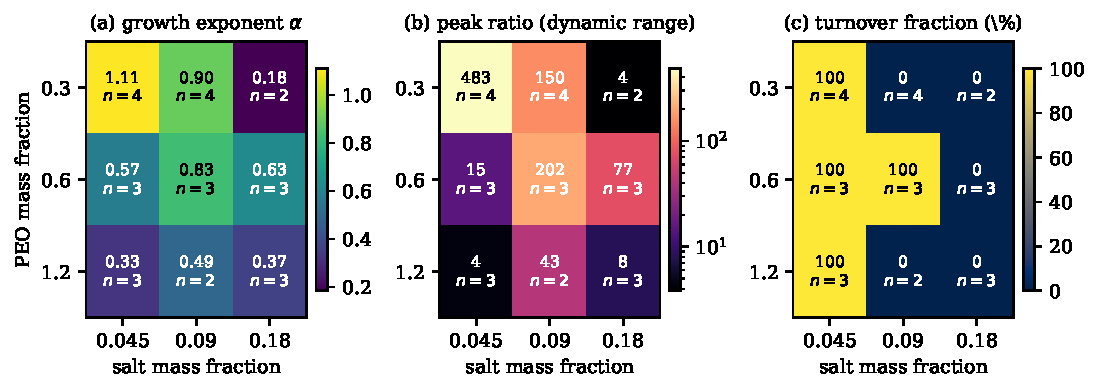
\includegraphics[width=\linewidth]{../figures/chapter3/potentiation_grid.pdf}
  \caption[Composition control of pulse-driven potentiation]{Potentiation (pulse-integration) response across the \SY{}/\PEO{}/\LiTf{} composition grid: (a) the log--log growth exponent $\alpha$, (b) the peak conductance ratio (usable dynamic range, log scale), and (c) the fraction of devices whose response turns over within the measured range ($N\le 1000$). Increasing the \PEO{} fraction lowers $\alpha$ and the dynamic range; increasing the salt fraction suppresses turnover, sustaining growth to higher pulse counts. Per-cell median, with the device count $n$ annotated in each cell.}
  \label{fig:ch3_potentiation}
\end{figure}

Taken together, these observations support a single physical reading: increasing the proportion of the ion-transport phase produces a weaker, faster-relaxing memristive response, while the salt content governs how far that response can be pushed before it saturates. This is the quantitative spine of the chapter, and the one result that rests on replicated devices.

%% ------------------------------------------------------------
\section{Chemical-Tuning Landscape}\label{sec:ch3_chemistry}
%% ------------------------------------------------------------

Beyond composition, the identity of the electrolyte components shifts the dynamics further. These comparisons are reported as an illustrative landscape: each matched cell (fixed composition, electrode, and protocol) contains at most one or two screened devices, so the magnitudes below are indicative and the sample size is given in every case.

\begin{figure}[t]
  \centering
  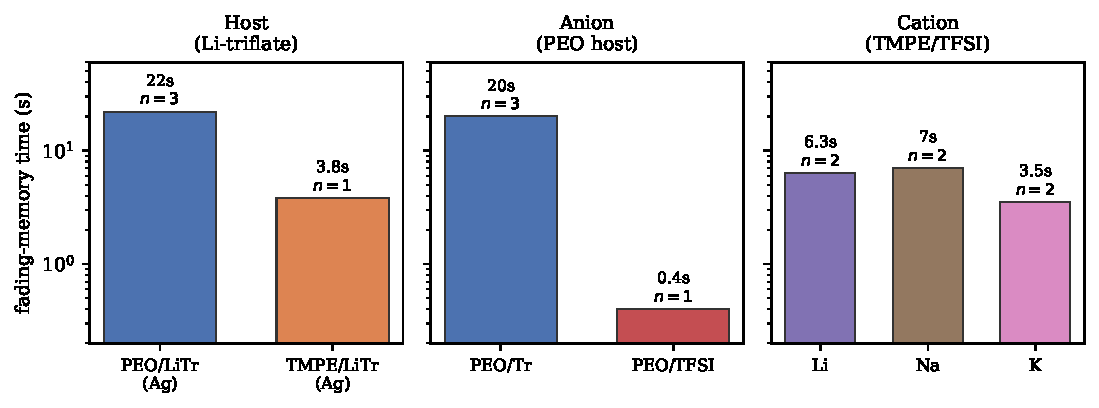
\includegraphics[width=\linewidth]{../figures/chapter3/chemistry_landscape.pdf}
  \caption[Chemical-tuning landscape of the fading-memory time]{Illustrative effect of electrolyte chemistry on the fading-memory time constant. Host and anion produce the largest shifts; the cation produces no consistent, host-independent ordering. Sample sizes are small (see text).}
  \label{fig:ch3_chemistry_landscape}
\end{figure}

\paragraph{Host.} Substituting the linear polyether \PEO{} by the hyperbranched polyether \TMPE{}, at fixed lithium-triflate chemistry and composition, shortens the fading-memory time by roughly a factor of six (\PEO{}/\LiTf{}: \(t_{1/2}\approx\SIrange{20}{25}{\second}\), three screened silver devices; \TMPE{}/\LiTf{}: \(\approx\SI{4}{\second}\), one screened silver device with a clear decay). This is the best-replicated of the chemistry comparisons and the clearest single chemistry effect, although the \TMPE{} side rests on a single clean device.

\paragraph{Anion.} Replacing triflate by the more charge-delocalised \TFSI{} anion, in the \PEO{} host, shortens the fading-memory time dramatically --- from \(\approx\SI{20}{\second}\) (triflate) to of order \SI{1}{\second} (\TFSI{}). The \TFSI{} decays additionally tend to a sharper, more abrupt (compressed) shape rather than the stretched form of the triflate devices, suggesting a qualitatively different relaxation-time distribution.

\paragraph{Cation.} The original motivating hypothesis --- that the alkali cation would order the fading-memory timescale as \ce{Li+} > \ce{Na+} > \ce{K+}, by analogy with the hard--soft acid--base argument of \cref{ch:poc}~\cite{Pearson1963} --- is \emph{not} supported by the data. The cleanest available cation comparison (the \TMPE{}/\TFSI{} family, two screened devices per cation in a single fabrication batch under the common protocol) places potassium shortest (\(t_{1/2}\approx\SI{3.5}{\second}\)) and lithium and sodium together and longer (\(\approx\SIrange{6}{7}{\second}\)); potassium being the shortest is consistent with the weakest cation--oxygen coordination, but lithium and sodium are not separable. Crucially, this ordering does not reproduce across families: in the triflate hosts the same cations give a different and even reversed ordering, and the within-cation device-to-device variation is comparable to the between-cation differences. The honest conclusion is that, in this archive, cation identity does not produce a robust, host- and anion-independent retention ordering. A properly powered test of the cation hypothesis would require a dedicated series at fixed protocol and electrode with at least three replicates per cell, and is identified as future work in \cref{sec:ch3_limitations}.

The hierarchy that emerges from this landscape is therefore that the host and the anion shift the fading-memory time more strongly, and more legibly, than the cation does.

%% ------------------------------------------------------------
\section{The Drive Protocol Sets the Timescale}\label{sec:ch3_protocol}
%% ------------------------------------------------------------

A methodological result underlies, and disciplines, every comparison above. Because the read voltage used to interrogate the state is above the ionic activation threshold, and because the write amplitude controls how far the ionic profile is driven, the \emph{drive protocol} itself influences the apparent fading-memory time. The point is made cleanly by a single device measured under both protocols: its fitted relaxation time increases from \(\approx\SI{4.6}{\second}\) under the \SI{3}{\volt}-write/\SI{1.5}{\volt}-read protocol to \(\approx\SI{15.5}{\second}\) under the \SI{6}{\volt}-write/\SI{3}{\volt}-read protocol --- a roughly three-fold change in the measured timescale with no change in material, only in drive.

\begin{figure}[t]
  \centering
  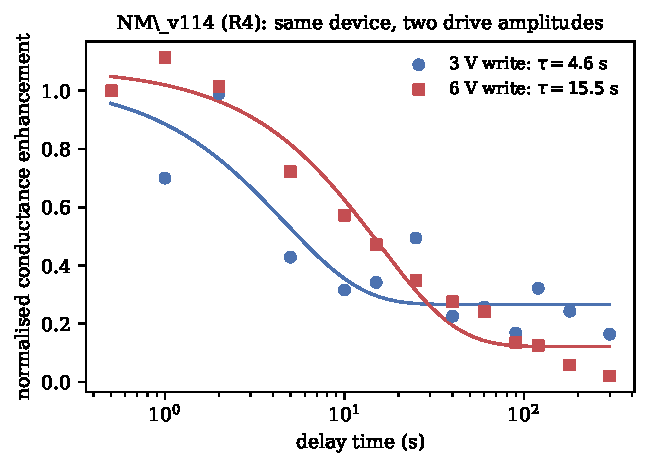
\includegraphics[width=0.62\linewidth]{../figures/chapter3/protocol_overlay.pdf}
  \caption[The drive protocol sets the apparent fading-memory time]{The apparent fading-memory time is set in part by the drive protocol. The same device, measured under a larger write/read amplitude, shows a markedly longer apparent relaxation time.}
  \label{fig:ch3_protocol}
\end{figure}

The mechanistic reading is that a larger write amplitude displaces more of the ionic charge (and, at the largest amplitudes, may drive electrode-level electrochemical processes), producing a deeper, longer-lived written state, while the supra-threshold read perturbs the state during interrogation. Two consequences follow. First, the composition result of \cref{sec:ch3_composition} is unaffected, because it was obtained entirely within a single, fixed protocol; only the chemistry comparisons, which unavoidably span device generations, are exposed to this confound, and they are reported accordingly. Second, the result is a positive design rule for the field: the volatile timescale of these devices is not a fixed material constant but is co-determined by how the device is driven, and any meaningful cross-device or cross-chemistry comparison of retention must hold the write/read protocol, the electrode, and the composition fixed.

%% ------------------------------------------------------------
\section{Discussion}\label{sec:ch3_discussion}
%% ------------------------------------------------------------

The picture that emerges is of a device whose volatile dynamics are controlled by a hierarchy of levers. The strongest and most reliable is the \emph{composition} of the ion-transport phase, which tunes the switching window, the potentiation strength, and the fading-memory time together and in the same direction: more ion-transport polymer yields a weaker, faster-relaxing device. Next come the \emph{host} and \emph{anion} of the electrolyte, which shift the fading-memory time over a wider range still but are documented here only illustratively. The \emph{cation}, which the proof-of-concept chapter's mechanism had suggested would be the controlling variable, is in fact the weakest and least legible lever in this dataset, and its effect is not separable from host, anion, and drive protocol at the available sample sizes. The hard--soft acid--base framework of \cref{ch:poc} is retained here as a qualitative organising idea --- it correctly anticipates, for instance, that the most weakly coordinating cation relaxes fastest within one family --- but it is explicitly not advanced as a quantitative, transferable law on the strength of these data.

The variability that runs through the chapter deserves a positive rather than an apologetic reading. The spread of fading-memory times, both across compositions (roughly an order of magnitude) and between nominally identical devices, is precisely the kind of heterogeneity that a physical reservoir requires: a bank of elements with diverse but individually reproducible-enough time constants. \Cref{ch:temporal} takes up this point directly.

%% ------------------------------------------------------------
\section{Limitations and Future Work}\label{sec:ch3_limitations}
%% ------------------------------------------------------------

The principal limitation is one of statistical power off the composition axis. Only the \SY{}/\PEO{}/\LiTf{} composition grid is replicated; the host, anion, and cation comparisons rest on one or two screened devices per matched cell, and are therefore illustrative. Three specific consequences should be stated plainly. First, the cation hypothesis is not tested here at adequate power, and the apparent absence of a \ce{Li+}>\ce{Na+}>\ce{K+} ordering should be read as ``not demonstrated in this archive'' rather than as a positive refutation. Second, the supra-threshold read and the amplitude dependence of the apparent timescale (\cref{sec:ch3_protocol}) mean that absolute retention values are protocol-specific. Third, electrode (silver versus gold) and ageing effects are additional uncontrolled variables that were held out rather than modelled. Fourth --- and most consequential for \cref{ch:temporal} --- pulse integration and forgetting were characterised \emph{separately}: the potentiation curves were all acquired at a single fixed inter-pulse interval (\SI{0.103}{\second}), while the fading-memory decays measure relaxation \emph{after} potentiation, so the archive contains no experiment that varies the input timing and thereby probes the interaction of integration and forgetting directly. The temporal-computing model of \cref{ch:temporal} must therefore \emph{compose} the measured input nonlinearity and the measured decay, and that composition is an explicit modelling assumption rather than a measured fact; a pulse-train experiment with systematically varied inter-pulse intervals is the natural way to test it.

The corresponding future-work programme is therefore well defined: a dedicated cation series in a single host and anion, at a single fixed protocol and electrode, with a sub-threshold read voltage (as in the proof-of-concept device of \cref{ch:poc}) and at least three replicates per cell, would convert the illustrative chemistry landscape into a powered comparison. Encapsulation and a systematic ageing study would address the stability dimension.

%% ------------------------------------------------------------
\section{Conclusions and Bridge to Chapter~4}\label{sec:ch3_bridge}
%% ------------------------------------------------------------

This chapter has shown that the volatile dynamics of \SY{}/polymer-electrolyte composites are controllable, and that the control is dominated by composition. Quantitatively, the fading-memory time of the \SY{}/\PEO{}/\LiTf{} system is tunable over roughly \SIrange{2}{20}{\second} by composition alone, with the switching window and potentiation strength varying in concert; chemistry (host, anion) extends this range further, illustratively; and the cation, contrary to the initial hypothesis, is not a robust controlling variable at the available power. A methodological result --- that the drive protocol co-sets the apparent timescale --- frames how all of this must be measured and compared.

What \cref{ch:temporal} requires from the present chapter is precisely a set of behavioural ingredients: a composition-indexed family of fading-memory time constants spanning a useful range, a characterisation of how conductance is built up by pulses (including its saturation and turnover), and an honest account of device-to-device heterogeneity. Those ingredients are now in hand. They also define the shape of the design space the next chapter inherits: the fading-memory time and the input nonlinearity ($\alpha$) are \emph{coupled} through the \PEO{} fraction --- a single composition selects a paired (memory, nonlinearity) operating point rather than two independent settings --- while the salt fraction acts as a partially separate lever on the usable dynamic range and turnover. A temporal-computing substrate must therefore be assembled from a \emph{bank} of compositions to span the behaviour it needs, rather than tuned to a single optimum; the heterogeneity catalogued here is what makes that bank possible. The next chapter treats them not as imperfections of a memory but as the raw material of a temporal-computing substrate.


%% ---- Standalone close (skipped when \include'd from thesis.tex) ----
%% A unified bibliography is printed from thesis.tex in the thesis build,
%% so the per-chapter \printbibliography runs only in standalone mode.
\ifdefined\thesismode
  \endinput
\fi

\printbibliography[heading=bibintoc, title={References}]
\end{document}
